\documentclass[11pt,letter]{article}

\usepackage{url}
\usepackage{hyperref}
\hypersetup{
   colorlinks,
   citecolor=Maroon,
   linkcolor=Maroon,
   urlcolor=blue
}
\usepackage{graphicx}
\usepackage[labelformat=simple]{subcaption}
\renewcommand\thesubfigure{(\alph{subfigure})}
\usepackage{algorithm, algorithmicx}
\usepackage{algpseudocode}
\usepackage{booktabs}
\usepackage{epstopdf}
\usepackage{natbib}
\usepackage{fullpage}
\usepackage{amsthm}

\algdef{SE}[EVENT]{Event}{EndEvent}[1]{\textbf{upon event}\ #1\ \algorithmicdo}{\algorithmicend\ \textbf{event}}%
\algtext*{EndEvent}

\algdef{SE}[PHASE]{Phase}{EndPhase}[1]{\textbf{Phase}\ #1\ \algorithmicdo}{\algorithmicend\}}%
\algtext*{EndPhase}

\algdef{SE}[PROCESS]{Process}{EndProcess}[1]{\textbf{Process}\ #1\ \algorithmicdo}{\algorithmicend\}}%
\algtext*{EndProcess}

\newcommand\todo[1]{{\color{red} {\bf TODO:} #1}}
\newtheorem{lemma}{Lemma}
\newtheorem{theorem}{Theorem}
\newcommand{\sol}{MAC}

\begin{document}

\title{\sol{}: Checkpoint-Restart for MPI}

\author{Rohan Garg}

\maketitle

\section{\sol{}: Design and Implementation}
\label{sec:design}

\subsection{To Do, or Not to Do: Checkpointing the MPI Library}

One approach to transparent checkpoint-restart of an MPI application
would be to save the state of the MPI library along with the application
state to a file on the disk; then, restore the MPI process, with the MPI
library state and the application, from the checkpoint file.

However, this requires the checkpointing package to recreate the underlying
network connections that the MPI library was using and in some cases to also
virtualize MPI library's access to the communication layer~\cite{caophdthesis}.

While one could extend the checkpointing package to support the wide variety
of HPC communication networks, this does require significant development
efforts, and is also not extensible to future HPC environments.

Since an MPI rank only communicates with other MPI ranks through the MPI API,
regardless of the underlying network, one could think of another transparent
checkpointing approach that tracks and virtualizes at the MPI API layer (for
example, by interposing on the MPI library calls).

However, this attempt also fails for several reasons. The MPI library state
that's saved and restored from the checkpoint file does not allow for
re-initialization (i.e., the MPI library initialization, \texttt{MPI\_Init()},
is non-reentrant). Furthermore, the communicators and topologies that existed
at checkpoint time, cannot be recreated and restored, since the MPI library
still retains pointers and state to those. While one could virtualize these
opaque identifiers, this does lead memory leaks, since there's no way to
reclaim or reuse these library internal structures.

Thus, \mpiSol{} takes a different approach: virtualizing and checkpointing at the
MPI API layer, while {\em not} saving and restoring the MPI library.
This is important to allow for replacement of an initialized MPI library
with a fresh, uninitialized one on restart.


The key idea is to ``split'' the
address space of the application process into two halves: an upper
half (which contains the application); and a lower half (which
contains the lh\_proxy, along with the non-reentrant library). The
library executing in the lower half (although in the same process's
address space) is not allowed to affect the memory of the upper
half. The lower half acts as an external lh\_proxy process -- it's
akin to running two processes in a single address space -- with its
own heap and stack. The assumption here is that there must be
be a strict API between the two halves. So, the two halves must
communicate only through this strict API.

This novel split-process approach allows \mpiSol{} to balance two
conflicting objectives: a shared address space (to avoid RPC and
data transfer overhead); and isolation (to avoid side-effects created
by a non-reentrant MPI library from leaking into the application's
address space). Note also that the lower half is expendable across
checkpoint-restart.

\subsubsection{Split-Process Approach: Expendable MPI Library}

To throw away regions of linked code at runtime (or across
checkpoint-restart), one requires the ability to robustly track and isolate
the memory regions being used by the different code segments, including any
side effects in a process's address space.

% TODO: Rephrase for clarity and conciseness
Dynamic linking enables one to dynamically load and link in arbitrary
pieces of code at runtime. The GNU toolchain provides API's, such as,
\texttt{dlopen}, \texttt{dlmopen}, to enable runtime, dynamic linking.

A first attempt at using the runtime linker/loader's dynamic loading
(e.g., \texttt{dlopen} and \texttt{dlmopen}) and unloading (e.g.,
\texttt{dlclose}) features fails for several reasons.

The fundamental issue is that these features were not intended for the
purpose of isolating different data or code segments, but rather for allowing
different, dynamically-loaded pieces of code to share the same address space,
including the process's heap and stack segments. Thus, it is very difficult
to robustly track and isolate memory regions being used by the different
code segments.

To get around this issue, one could try to use the \texttt{dlclose} function
of the runtime linker/loader to unload the region of code that one wants to
throw away. But this fails to provide the isolation we want. Note that dynamic
loading and linking depends on a destructor function implemented in a library
to clean up any remnants at unload time. A destructor that can clean up
all of the library's side effects in memory is often difficult to write and
fundamentally impossible in many cases~\cite{garg2018crum}. Thus, this approach
not only leads to memory leaks but a freshly loaded library can fail to
initialize if it finds any inconsistent state in process's
memory~\cite{garg2018crum}.

Finally, even with a destructor that can clean up a library's side effects in
process's memory, it's difficult to handle saving and restoring of the
state of an ``external'' subsystem that the library may be interacting with.
For example, the MPI library often talks to an MPI process manager to
enquire about global state, such as, the MPI rank of the current process.

Therefore, \mpiSol{} uses the following approach for isolating the MPI library
in an MPI process. The key idea is to have two separate runtime loaders,
each with its separate heap and stack. Recall that there's just one runtime
loader per process in a Linux process, which is loaded at process startup time
the Linux kernel. The loader is responsible for loading in all the dependencies
of the target executable and runtime symbol resolution (using the PLT).

So, \mpiSol{} emulates what the kernel does at process startup: sets up a new
stack segment, a new heap segment, loads in a second runtime linker/loader,
and finally ``asks'' the second copy of the runtime linker/loader to load
in the MPI library. \mpiSol{} keeps track of memory regions of the second runtime
linker/loader creates by interposing on its \texttt{mmap} calls.
Also, since the second ld.so is only aware of the new heap and stack,
this is what it and the libraries it loads will continue to use.

Since the side effects of the MPI library are now restricted to ``known''
memory regions, there are no memory leaks and these side effects cannot
creep and pollute the application's memory regions. This allows \mpiSol{} to
easily throw away all of these ``known'' memory regions across
checkpoint-restart. On restart, \mpiSol{} loads in a new runtime loader
with a new heap and stack and initializes it again.

Another advantage of this approach is that this is completely transparent
to the end-user application and requires no modifications to the runtime
loader, the Linux kernel, the application, or any library.

This approach allows \mpiSol{} to efficiently interpose and virtualize at
the MPI API layer, and at the same time, allow for replacement of an
initialized MPI library with a fresh, uninitialized one on restart.

A typical MPI application consists of distributed processes (MPI ranks)
that can create subgroups for communication, send messages to each other,
and invoke global barriers and do collective communication. Next, we discuss
how \mpiSol{} saves and restores these three important components of an MPI
computation.

\subsection{Checkpointing MPI Communicators, Groups, and Topologies}

An MPI application can create communication subgroups and topologies for
connecting groups of processes for ease of programmability and for efficient
communication. MPI implementations provide opaque handles to the application
as a reference to a communicator object or group.

\mpiSol{} interposes on all rhe calls that refer to these opaque identifiers,
and virtualizes the identifiers. At runtime, \mpiSol{} records any MPI calls
that can modify the MPI communication state, such as \texttt{MPI\_Comm\_create},
\texttt{MPI\_Group\_incl}, etc.  On restart, \mpiSol{} recreates the MPI
communicator state by replaying the MPI calls using a new MPI library. So,
while the new MPI library may provide different opaque identifiers, the
runtime virtualization allows the application to continue to run with
consistent handles across checkpoint-restart.

A similar checkpointing strategy also works for other opaque identifiers, such
as, MPI derived datatypes, etc.

\subsection{Checkpointing MPI Point-to-Point Communication}

The next challenge in checkpointing MPI computations is the problem of
saving the network state.

Capturing the state of MPI processes requires quiescing the process threads,
and preserving the process memory to a file on the disk. However, this alone
is not sufficient to capture a consistent state of the computation. Any MPI
messages that were already sent but not yet received at the time of quiescing
all the processes must also be saved as part of the checkpoint.

\begin{figure*}[t!]
  \centering
  \begin{subfigure}[t]{0.20\textwidth}
    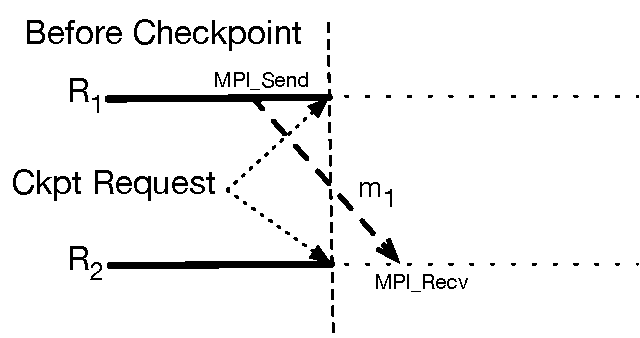
\includegraphics[scale=0.38]{figures/mpiDrainAlgo1}
    \caption{No draining of in-flight messages at checkpoint time.}
  \end{subfigure}\hfill%
  \begin{subfigure}[t]{0.20\textwidth}
    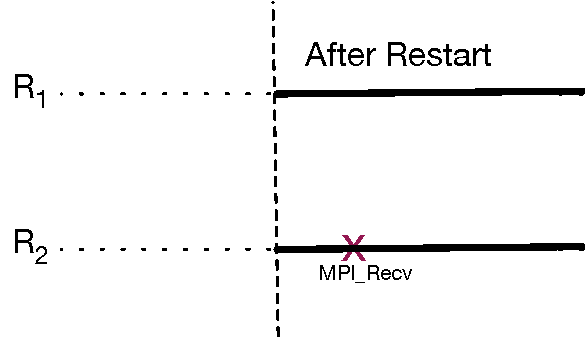
\includegraphics[scale=0.38]{figures/mpiDrainAlgo2}
    \caption{Failed \texttt{MPI\_Recv} on restart.}
  \end{subfigure}\hfill%
  \begin{subfigure}[t]{0.20\textwidth}
    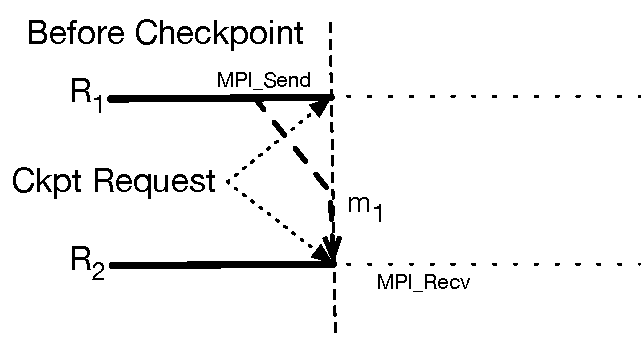
\includegraphics[scale=0.38]{figures/mpiDrainAlgo3}
    \caption{\sol{} drains in-flight messages.}
  \end{subfigure}\hfill%
  \begin{subfigure}[t]{0.20\textwidth}
    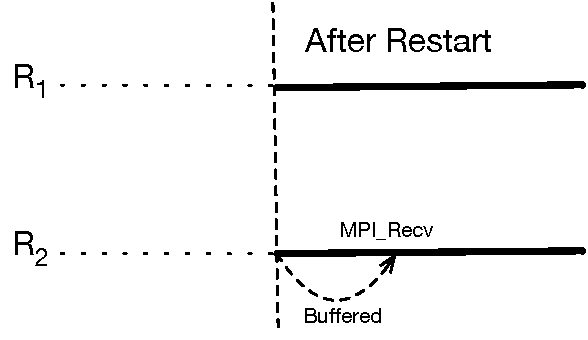
\includegraphics[scale=0.38]{figures/mpiDrainAlgo4}
    \caption{\sol{} returns the buffered in-flight messages on restart.}
  \end{subfigure}
  \caption{Checkpointing MPI point-to-point communication.\label{fig:inFlightMsgs}}
\end{figure*}

Figure~\ref{fig:inFlightMsgs} shows the state of a system with two MPI ranks,
$R_1$ and $R_2$. Rank $R_1$ sends a message, $m_1$, to rank $R_2$ and then,
receives a checkpoint request from the user. On the other hand, rank $R_2$
receives the checkpoint request before it can receive the message, $m_1$.
If the state of the network channel, with the message, $m_1$, is not saved,
this can lead to a deadlock on restart. This is because when rank $R_1$ is
restored from the same point on restart, it remembers that it had sent
the message in the ``past'' and it's not going to send the message again;
and since rank $R_2$ had not received the message at checkpoint time, it's
going to get stuck when it resumes to do the receive on restart.

% This is further complicated by the use of asynchronous MPI communication
% primitives.

Thus, \mpiSol{} uses a novel MPI message draining algorithm to save all
{\em in-flight} MPI messages to capture the state of the network. The main
idea is to publish local information (send/receive counts, and pending
sends) to a centralized key-value database, and iterate until all unreceived
messages have been received and buffered. Algorithm~\ref{algo:mpiDrainAlgo}
describes the algorithm in more detail.

\begin{algorithm}
  \begin{algorithmic}[1]
    \caption{\label{algo:mpiDrainAlgo} Algorithm for MPI message draining.}
      \Event{Checkpoint request}
        \ForAll{R $\in$ MPI Ranks}
          \State{pendingSends $\gets$ GetLocalPendingSends()}
          \State{PublishLocalSendsAndRecvCounts(pendingSends)}
          \State{GlobalBarrier()}
          \State{$<$totalSends, totalRecvs$>$ $\gets$ GetGlobalCounts()}
          \While{totalSends $>$ totalRecvs}
            \State{DrainPackets(pendingSends)}
            \State{GlobalBarrier()}
            \State{pendingSends $\gets$ GetLocalPendingSends()}
            \State{PublishLocalSendsAndRecvCounts(pendingSends)}
            \State{$<$totalSends, totalRecvs$>$ $\gets$ GetGlobalCounts()}
          \EndWhile
        \EndFor
      \EndEvent
      \Function{GetLocalPendingSends}{}
        \State{pendingSends $\gets \emptyset$}
        \ForAll{s $\in$ MPI Asynchronous Send Requests}
          \If{MPI\_Test(s) $=$ Success}
            \State{pendingSends $\gets$ pendingSends $\cup$ \{s\}}
          \EndIf
        \EndFor
        \State{\Return{pendingSends}}
      \EndFunction
      \Procedure{DrainPackets}{pendingSends}
        \ForAll{s $\in$ pendingSends}
          \If{MPI\_Iprobe(s) $=$ Success}
            \State{MPI\_Recv(s, localBuffer)}
            \State{UpdateLocalRecvCount()}
          \EndIf
        \EndFor
      \EndProcedure
  \end{algorithmic}
\end{algorithm}

At runtime, \mpiSol{} keeps track of message send and receive requests to MPI. In
particular, it tracks the blocking, synchronous, and asynchronous send and
receive requests. Note that the only information that's tracked is the number
of such requests and some additional metadata (like the communicator and
datatype); the message contents are not tracked. This allows \mpiSol{} to compute
the global set of pending sends at each rank at any given point in time.

At checkpoint time, first, each rank publishes its local counts and set of
pending (unreceived) sends to a centralized key-value database. Second, each
rank receives the information for all the ranks through the centralized
database. Third, each rank locally probes and tries to receive the unreceived
sent messages. If the receive is successful at a rank (meaning that some rank
had sent it a message prior before the checkpointing request arrived),
the rank updates its local receive count. Finally, each rank loops through
the same set of these three steps, until the global send count becomes less
than or equal to the global receive count and there are no more unreceived
sent messages. (Note that the receive count can be higher than the send
count, since a rank might post receive requests even before any message has
been sent.)

After resuming from a checkpoint, any receive requests by the application
are matched against the receive requests that were completed during the
execution of Algorithm~\ref{algo:mpiDrainAlgo} (at checkpoint time) and
returned locally.

\begin{theorem}
  Algorithm~\ref{algo:mpiDrainAlgo} finishes without deadlocks, assuming
  a loss-free network.
\end{theorem}

\begin{proof}
  If the total receive count is higher than the total send count, and there
  are no pending sends, then there are no in-flight messages to drain.

  None of the MPI calls used in draining of messages can block indefinitely
  (assuming a loss-free network). Also, the call to \texttt{MPI\_Recv()} in
  the \texttt{DrainPackets()} function must also not block, since the only
  reason it was executed was because the earlier \texttt{MPI\_Iprobe()} call
  was successful. The MPI standard guarantees that the receive will not block
  if the probe was successful.

  Since at each iteration of the main loop, the total receive count can
  only increase, eventually, the control must break out of the loop.
\end{proof}

\subsection{Checkpointing MPI Collectives}

The next challenge in checkpointing of MPI applications is about handling
the MPI barriers and collective communication.

MPI collective communication primitives involve communication amongst all or
a program-defined subset of MPI ranks. These are typically implemented using
the concepts of global barriers among distributed processes.

The semantics of a barrier (or collective call) only guarantees that none of
the processes can exit out of a barrier until all of them have entered into the
barrier. There are no guarantees on when and in what order they'll exit out
of the barrier.

These semantics create some interesting challenges for checkpointing MPI
applications.

\noindent \textbf{Challenge I: Straggler Ranks} A rank stuck in some
computation cannot release another rank that had already entered into a barrier
where both the ranks are participants. We call the rank that's lagging behind
in the computation a {\em straggler rank}.

If a checkpoint request were to arrive at this point, it's unclear how one
would restore the state of the MPI computation, without leading to an
inconsistent state or a deadlock.

One possibility is to log calls to the barrier and remove the call log when
exiting out of the barrier and allow ranks to be interrupted out of a barrier
for a checkpoint. However, this approach leads to a deadlock on restart, if a
checkpoint message is seen after exiting out of the barrier but before the
call log can be removed by some rank, while for all the other ranks, the
checkpoint message is seen after they have removed the call log. This is
because, on restart, the rank that was checkpointed before the call log
was removed, would end up re-executing the barrier call and would get stuck,
since all other ranks had already exited out of the barrier.

Another related issue is the problem of a domino effect, which is described
next.

\noindent \textbf{Challenge II: Domino Effect}  A na{\"i}ve approach that
waits for all processes to exit out of a barrier can lead to a domino effect
and an indefinite wait for a checkpoint to ever take place. This is because
there's no principled way to wait for all processes to exit out of a barrier
and take a checkpoint. A rank that's participating in multiple barriers, could
exit out of the first barrier (assuming all its peers had entered into the
first barrier), race ahead and enter into the second barrier, before it gets
to see the checkpoint request.

\begin{figure}[t!]
  \centering
  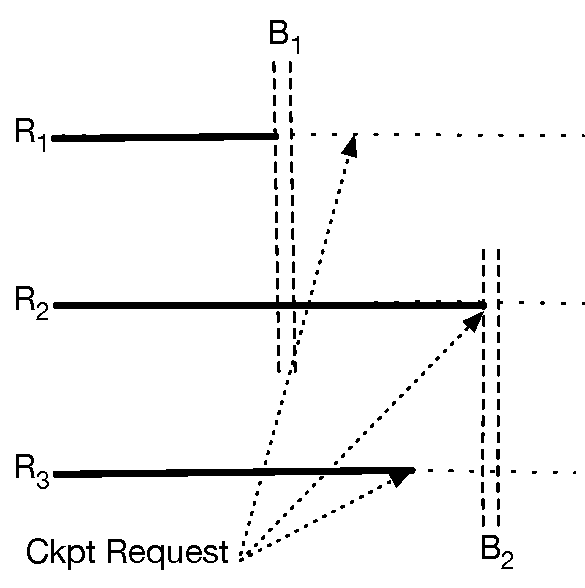
\includegraphics[scale=0.5]{figures/mpiDominoEffect}
  \caption{Domino effect with checkpointing of MPI collective
  communication.\label{fig:dominoEffect}}
\end{figure}

Figure~\ref{fig:dominoEffect} illustrates this problem with three MPI ranks:
$R_1, R_2,$ and $R_3$. Ranks $R_1$ and $R_2$ enter into a barrier, $B_1$. Rank
$R_2$ exits out of the barrier, and enters into the second barrier, $B_2$, where
it gets blocked because rank $R_3$ is stuck in some computation. The checkpoint
request arrives after rank $R_2$ enters into $B_2$. Now, there are three
choices: (a) wait for rank $R_2$ to exit out of barrier before checkpointing,
$B_2$; or, (b) interrupt the rank out of the barrier and checkpoint; or, (c)
abandon the checkpoint.

If one were to choose option (a), then this results in a deadlock. This
is because rank $R_3$ had received the checkpoint message before it had entered
into the barrier and now cannot proceed (since it is quiesced).

On the other hand, if one were to choose option (b), then at checkpoint time,
it violates the invariant that checkpointing shall not take place while a
rank is in a barrier. Note that this invariant is important, since otherwise,
it can lead to a situation where we take a checkpoint when all of the ranks
had entered into a barrier, but any of the ranks was yet to exit out of the
barrier. It's unclear how one would restore the state of the MPI computation in
this case using just the MPI API: one must choose to either to re-execute
the barrier call for all the ranks, or for none of the ranks, leading to
inconsistent state in some cases and deadlocks in some other cases, depending
on exactly when the checkpoint request was seen).

Finally, if one were to choose option (c), this can lead to a domino effect
with multiple overlapping barriers, resulting in no checkpoint ever taking
place.

\noindent \textbf{Key Idea:} To address the two challenges listed above, \mpiSol{}
uses a novel two-phased checkpointing algorithm that ensures that all MPI
collectives and barriers are turned into {\em interruptible and restart-able}
collectives.

The algorithm employs four key techniques:

\begin{itemize}
  \item A central, coordinator process, which does not participate in the
        checkpointing, but assists in keep track of the global state.

  \item Each MPI collective call is decomposed into two barriers: a trivial
         barrier, and the real MPI collective call. The first barrier (trivial
         barrier) allows \mpiSol{} to checkpoint even in the presence of
         straggler ranks; the first barrier can be thrown away on restart.

  \item Checkpointing is divided into two phase: in the first phase, a
        checkpoint ``intent'' message is sent; and, in the second phase, when
        all the ranks agree on having reached a safe state, the checkpoint
        message is broadcasted to all the ranks. This allows \mpiSol{} to
        avoid the problem of domino effect, since once a checkpoint-intent
        message is received by a rank, it cannot race ahead and enter into a
        second barrier, without coordinator's explicit permission (``free
        pass'').

  \item A checkpoint helper thread in each rank allows \mpiSol{} to inspect the
        current state of the rank and communicate with the central coordinator.
\end{itemize}

Algorithm~\ref{algo:mpi2pc} describes the protocol in further details.

\begin{algorithm}
  \begin{algorithmic}[1]
    \caption{\label{algo:mpi2pc} Algorithm for deadlock-free checkpointing of MPI collectives.}
    \Process{MPI Rank}
      \State{state $\gets$ Ready}
      \Function{MPI Collective Wrapper}{}
       \State{inCollectiveWrapper $\gets$ True}
       \If{CkptIntentRecvd()}
         \State{state $\gets$ Phase-1; WaitForFreePass()}
         \If{CkptMsgRecvd()}
           \State{WaitForCkptSignal()}
         \EndIf
       \EndIf
       \State{Atomically: state $\gets$ TrivBarrier; ExecuteMpiBarrier()}
       \If{CkptIntentRecvd()}
         \State{state $\gets$ Phase-2; WaitForFreePass()}
         \If{CkptMsgRecvd()}
           \State{WaitForCkptSignal()}
         \EndIf
       \EndIf
       \State{Atomically: state $\gets$ Collect; ExecuteMpiCollective() \label{line:collective}}
       \State{state $\gets$ Ready; inCollectiveWrapper $\gets$ False}
      \EndFunction
    \EndProcess
    \algstore{part1}
  \end{algorithmic}
\end{algorithm}
\begin{algorithm}
  \begin{algorithmic}[1]
    \algrestore{part1}
    \Process{Checkpoint helper thread (in each MPI Rank)}
      \Event{Checkpoint Intent}
        \State{SetCkptIntentRecvd() \label{line:setCkptIntent}}
      \EndEvent
      \Event{Free Pass}
        \State{SetFreePass()}
      \EndEvent
      \Event{Checkpoint Message}
        \State{SetCkptMsgRecvd()}
        \State{SetFreePass()}
        \State{RaiseCheckpointSignal()}
      \EndEvent
      \If {inCollectiveWrapper}
        \State{WaitForRankToReachASafeState() \label{line:waitForSafePoint}}
      \EndIf
      \State{SendCurrentStateToCoordinator() \label{line:reportToCoord}}
    \EndProcess
    \algstore{part2}
  \end{algorithmic}
\end{algorithm}
\begin{algorithm}
  \begin{algorithmic}[1]
    \algrestore{part2}
    \Process{Checkpoint Coordinator}
      \State{SafeStates $\gets$ \{Ready, Phase-1, TrivBarrier, Phase-2\}}
      \State{BcastCkptIntentToAllRanks(); ckptPending $\gets$ True\label{line:bcastIntent}}
      \While{ckptPending}
        \State{resps $\gets$ WaitForResponsesFromAllRanks() \label{line:waitForResponses}}
        \If{resps[r] $\in$ SafeStates, $\forall$ r $\in$ Ranks}
          \State{BcastCkptMsgToAllRanks(); WaitForCkpt() \label{line:bcastCkpt}}
          \State{ckptPending $\gets$ False}
        \EndIf
        \If{resps[r] $\notin$ Collect, $\forall$ r $\in$ Ranks}
          \State{continue}
        \EndIf
        \ForAll{r $\in$ Ranks}
          \If{resps[r] $\in$ \{Phase-2\}}
            \State{SendFreePass(r) \label{line:sendFreePass}}
          \ElsIf{resps[r] $\in$ \{Ready, Collect, TrivBarrier\}}
            \State{GetStatus(r)}
          \EndIf
        \EndFor
      \EndWhile
    \EndProcess
  \end{algorithmic}
\end{algorithm}

 At run time, \mpiSol{} interposes on each collective call and executes the
 collective call in two steps: a dummy (trivial) MPI barrier, and the real
 collective communication call. A separate checkpoint helper thread is also
 injected into each rank. This thread is responsible for listening to different
 checkpoint-related messages from a coordinator process. The coordinator
 process does not participate in the checkpointing directly.

 At checkpoint time, the coordinator process, broadcasts a checkpoint intent
 message to all the connected ranks (Line~\ref{line:bcastIntent}). The
 checkpoint thread in each rank sets a global variable
 (Line~\ref{line:setCkptIntent}), waits for application thread to reach a
 ``safe'' point (Line~\ref{line:waitForSafePoint}), and then reports to the
 coordinator with the current state of the rank (Line~\ref{line:reportToCoord}).

 The coordinator waits for responses from all the ranks
 (Line~\ref{line:waitForResponses}). If all the ranks respond with ready
 status, the coordinator broadcasts the actual checkpoint
 request (Line~\ref{line:bcastCkpt}). A rank is deemed to be in a safe state for
 checkpointing, if it is in any of the following states: Phase-1, Phase-2,
 Ready, or TrivBarrier (i.e., in the trivial barrier).

 If any rank has entered into the real collective call
 (Line~\ref{line:collective}), the coordinator cannot proceed with
 checkpointing.  The coordinator must then allow all the ranks to get enter into
 and then exit from the collective call to proceed with checkpointing.
 It does so by sending ``free pass'' to all the ranks that are stuck in Phase-2
 (Line~\ref{line:sendFreePass}). Note that there
 can be no straggler ranks in this case (ranks that have yet to enter the
 wrapper function or are stuck in Phase-1), since the only way some rank can
 enter into the collective call is if all the ranks have at least entered
 the trivial barrier.

 After sending a free pass to all the ranks stuck in Phase-2, the coordinator
 waits for the next round of responses, when all the ranks exit from the
 collective call become ready for checkpointing. Note that even if some
 rank were to race ahead at this point and enter into another collective
 wrapper, the rank would get blocked in Phase-1 (of the second collective call).
 This prevents the problem of the domino effect. Eventually, all ranks stop at
 a safe point.

 Thus, at checkpoint time, all ranks are guaranteed to be outside the
 collective call.

 At restart time, all ranks skip the trivial barrier in the collective call
 wrapper function where some ranks were stuck at checkpoint time and directly
 execute the real collective call. This ensures a consistent state of the
 computation on restart.

\begin{theorem}
  Algorithm~\ref{algo:mpi2pc} ensures deadlock-free checkpointing for MPI
  collectives and barriers, without domino effect.
  (Assumption: We assume a loss-free network.)
\end{theorem}

\begin{proof}
  If even one rank passes the trivial barrier, then all ranks
  participating in that collective call can finish the corresponding
  collective call without hitting a deadlock.

  If even one rank enters into the collective call, then all ranks have,
  at least, entered the trivial barrier. They'll eventually exit out of the
  trivial barrier and get stuck in Phase-2, or enter into the collective call
  (assuming the checkpoint intent message was not seen in time).

  Once a checkpoint intent message is broadcasted, each rank will either get
  stuck in Phase-1 or in Phase-2 and cannot proceed until the coordinator
  sends a free pass.

  The coordinator sends a free pass only if a rank had entered into the
  collective call before it got a chance to see the intent message. But this
  implies that all the ranks participating in that collective call have entered
  into the trivial barrier. That is, there can be no stragglers. In this case,
  any ranks that get stuck in Phase-2, can be released and eventually, they'll
  all exit out of the collective call.

  Finally, in the presence of straggler ranks, any rank that is not a straggler
  will get stuck either in Phase-1 or in in the trivial barrier, depending on
  when the intent message arrives. For ranks that are stuck in the trivial
  barrier, the barrier can be interrupted and simply be skipped on restart.
\end{proof}

To gain further confidence in our implementation, we developed a model for the
protocol in TLA+~\cite{lamport1999tla} and used the TLA+ model checker to
verify the algorithm invariants of deadlock-free execution and consistent
state with multiple concurrently executing MPI processes. The TLA+ model checker
did not report any deadlocks or broken invariants for our implementation.

\bibliographystyle{plain}
\bibliography{design}

\end{document}
